\section{Theoretical Background} \label{theory}

This chapter deals with the past and present research in the relevant area which include literature review. This includes 
the significance of precise modelling of the ship's speed and its subsequent use in forecasting the ship's operation.
The theoretical background of Random Forest Regression will be discussed in this chapter. 

\subsection{Literature Review}\label{litreview}

The work by Yan et al. \cite{Yan.2021} provides a thorough review of the different attempts that have been made by different authors  to predict different parameters of ship's operation, this includes ship's fuel consumption. Per definition by Haranen et al. \cite{MichaelHaranen.2016}, the modelling of ship operation is categorised into White Box Model (WBM), Black Box Model (BBM) and Grey Box Model (GBM). Machine learning approach is categorised as BBM, BBM approach is defined as purely data driven approach requiring no prior knowledge about the ship operation. The literature review by Yan et al. \cite{Yan.2021} indicated that about $42\%$ of the research utlised BBM model based on machine learning approach.\\ 

Majority of the BBM approach based on ML is dominated by ANN \cite{Yan.2021}. However, there are works that considered decision tree-based modelling approach such as Decision Tree (DT), Random Forest (RF) and Extra Tree (ET). Soner et al. \cite{Soner.2018} implemented tree-based model, which include bagging, random forest (RF), and bootstrap, using data captured from onboard sensors of a ferry to predict speed through water and fuel consumption per hour. From the test dataset, the random forest model reported root mean square error (RMSE) of $0.34$ Knots during its prediction of Speed Through Water (STW). Yan et al. \cite{Yan.2020} used random forest (RF) model to minimise fuel consumption for a voyage of a dry bulk ship. The model use ship operational data and sea and weather data from noon report and EMCWF. The prediction performance report from this literature revealed mean absolute percentage error (MAPE) of $7.91\%$.\\      

The research by Gkerekos et al. \cite{Gkerekos.2019} highlighted the performance of different machine learning models to predict ship's fuel consumption per day using both noon data and automated data logging and monitoring (ADLM) system from a bulk carrier. This research concludes that tree based model displayed good prediction performance on both noon data and sensor based data. Using default parameters, RF model obtained $R^2$ score of $87.55\%$ and $96.26\%$ for noon data datasets and sensor-based data respectively. It is also noted that it that the data from a 3-month period in ADLM system would be sufficient to create a model with better performance than the model generated by noon data from a collection period of 2.5 year. This literature also concluded that automatic sensor-based data have the potential to increase the model accuracy score, $R^2$, by $5-7\%$.\\

Li et al. \cite{Li.2022} performed more extensive research on the effects of data fusions between meteorological data, ship voyage data and AIS data on different machine learning models to predict the ship's FOC. This research highlighted the advantage of fusing meteorological data and ship voyage data. The evaluation on different model performance indicated that RF are among preferable model candidate that could be used in commercial scale due to its good prediction capability and robustness against different datasets. The model performance comparison in their work reported $R^2$ score are above $96\%$ when deployed on the best datasets and achieved $R^2$ score in range between $74\% - 90\%$ over test data. The findings from their work also indicated the robustness of RF, as it displayed the lowest standard deviation at $0.015$ of the $R^2$ score when evaluated against random splits of datasets.\\

Abebe et al. \cite{Abebe.2020} used different approach in their research by predicting the ship's Speed Over Ground (SOG) instead of FOC. In this work, AIS data and noon-report weather data from 14 tracks and 62 ships are used for the SOG prediction. This literature reported that for random forest regressor (RFR), It achieved root mean squared error RMSE of $0.25$ knots using $489$ seconds for training. While decision tree achieved RMSE of $0.36$ knots taking up $52$ seconds for training. This shows that RFR outperforms DTR at cost of computational power.\\

This literature review indicated the capability of Random Forest Regressor to predict fuel consumptions and ship speed, irrespective of data source and type of data used. Promising results from different performance measures across different literatures indicated the capability random forest model as predictor. This brings us to RQ2 described in chapter \ref{objectives}: how can we extract maximum prediction performance from random forest. Due to the nonlinear, third order function estimate of fuel consumption described in chapter \ref{introduction} by Ronen \cite{Ronen.1982}. Accurate prediction of ship speed is necessary to ensure optimal operation and increase profitability. 

\subsection{Random Forest Regressor (RFR)}\label{rfrtheo}

% {Bal Be{\c{s}}ik{\c{c}}i}

\begin{figure}[h]
\centering
\begin{minipage}[b]{.5\textwidth}
    \centering
    \begin{tikzpicture}[x=0.75pt,y=0.75pt,yscale=-1,xscale=1]
    %uncomment if require: \path (0,433); %set diagram left start at 0, and has height of 433
    
    %Shape: Square [id:dp5731268858272198] 
    \draw   (180,110) -- (370,110) -- (370,300) -- (180,300) -- cycle ;
    %Straight Lines [id:da615072570759449] 
    \draw    (250,110) -- (250,300) ;
    %Straight Lines [id:da8002566967918264] 
    \draw    (300,110) -- (300,300) ;
    %Straight Lines [id:da4409034763483005] 
    \draw    (180,230) -- (250,230) ;
    %Straight Lines [id:da07514682530914596] 
    \draw    (300,170) -- (370,170) ;
    
    % Text Node
    \draw (131,192.4) node [anchor=north west][inner sep=0.75pt]    {$X_{2}$};
    % Text Node
    \draw (261,340.4) node [anchor=north west][inner sep=0.75pt]    {$X_{1}$};
    % Text Node
    \draw (157,222.4) node [anchor=north west][inner sep=0.75pt]    {$t_{2}$};
    % Text Node
    \draw (201,252.4) node [anchor=north west][inner sep=0.75pt]    {$R_{1}$};
    % Text Node
    \draw (201,162.4) node [anchor=north west][inner sep=0.75pt]    {$R_{2}$};
    % Text Node
    \draw (268,192.4) node [anchor=north west][inner sep=0.75pt]    {$R_{3}$};
    % Text Node
    \draw (321,132.4) node [anchor=north west][inner sep=0.75pt]    {$R_{4}$};
    % Text Node
    \draw (321,220.4) node [anchor=north west][inner sep=0.75pt]    {$R_{5}$};
    % Text Node
    \draw (241,310.4) node [anchor=north west][inner sep=0.75pt]    {$t_{1}$};
    % Text Node
    \draw (291,312.4) node [anchor=north west][inner sep=0.75pt]    {$t_{3}$};
    % Text Node
    \draw (381,162.4) node [anchor=north west][inner sep=0.75pt]    {$t_{4}$};
    
    \end{tikzpicture}
    
    \captionof{figure}{Example of partition space} 
    \label{fig:partitionspace}
\end{minipage}%
\begin{minipage}[b]{.5\textwidth}
    \centering
    \begin{tikzpicture}
        \tikzset{level distance=65pt,sibling distance=10pt,edge from parent/.style=
        {draw,edge from parent path={(\tikzparentnode.south)
                                -- +(0,-8pt)
                                -| (\tikzchildnode)}}}
    \Tree [.$X_1\leq t_1$ [.$X_2\leq t_2$ [.$R_1$ ] [.$R_2$ ] ]
        [.$X_1\leq t_3$ [.$R_3$ ]
        [.$X_2\leq t_4$ [.$R_4$ ] [.$R_5$ ] ] ] ]
    \end{tikzpicture}
    \captionof{figure}{Example of partition tree} 
    \label{fig:partitiontree}
\end{minipage}
\end{figure}


\begin{tikzpicture}[x=0.75pt,y=0.75pt,yscale=-1,xscale=1]
    %uncomment if require: \path (0,452); %set diagram left start at 0, and has height of 452
    
    %Shape: Axis 2D [id:dp697661158302031] 
    \draw  (220,297.8) -- (517.5,297.8)(249.75,80) -- (249.75,322) (510.5,292.8) -- (517.5,297.8) -- (510.5,302.8) (244.75,87) -- (249.75,80) -- (254.75,87)  ;
    %Image [id:dp23308396965327827] 
    \draw (245,305) node [rotate=-40.58] {
\includegraphics[width=26.87pt,height=72.39pt]{02_figures/ferry.jpg}};
    
    
    
    
\end{tikzpicture}

Suppose the following decision tree regressor


\subsection{Ship speed}


\subsection{Modelling}




